\documentclass[11pt,a4paper]{article}
\usepackage[utf8]{inputenc}
\usepackage[T1]{fontenc}
\usepackage[english]{babel}
\usepackage{lmodern,microtype,amsmath,amssymb,booktabs,array,graphicx,xcolor,geometry,setspace,float,longtable}
\usepackage{tikz}
\usetikzlibrary{arrows.meta,positioning}
\usepackage[font=small,labelfont=bf]{caption}
\usepackage[hidelinks]{hyperref}
\geometry{margin=25mm}
\setstretch{1.16}
\setlength{\parskip}{0.35em}
\setlength{\parindent}{1.2em}
\setlength{\emergencystretch}{2em}
\makeatletter
\setlength{\@fptop}{0pt}
\setlength{\@fpsep}{18pt}
\setlength{\@fpbot}{0pt plus 1fil}
\makeatother
\definecolor{reused}{HTML}{1755A0}
\definecolor{revised}{HTML}{B85A00}
\definecolor{added}{HTML}{B02228}
\newcommand{\old}[1]{{\color{reused}#1}}
\newcommand{\rev}[1]{{\color{revised}#1}}
\newcommand{\new}[1]{{\color{added}#1}}
\newenvironment{addition}{\begingroup\color{added}}{\endgroup}
\newcommand{\pp}{percentage points}
\newcommand{\figroot}{../../3. Output/paper_B/figures/}
\newcommand{\draftlegend}{\begin{center}\small\color{black}Coauthor working draft --- 22 September 2026\\\old{Blue: wording retained verbatim.}\quad\rev{Orange: revised existing material.}\\\new{Red: new text or analysis.} Figure frames and captions indicate provenance; plotted colors do not.\end{center}}
\newcommand{\authors}{\old{Ignacio Garijo-Campos} \and \old{Antonio Alfonso} \and \old{Pablo Bra\~nas-Garza} \and \old{Diego Jorrat} \and \old{Angel Sanchez}}
\newcommand{\plot}[4]{\begin{figure}[!htbp]\centering\begingroup\color{#1}\setlength{\fboxsep}{2pt}\fbox{\includegraphics[width=.94\linewidth]{\figroot#2.png}}\caption{\textcolor{#1}{#3}}\label{#4}\endgroup\end{figure}}
\newcommand{\tabnote}[1]{\par\smallskip{\footnotesize\noindent\textit{Notes:} #1\par}}
\newcommand{\inputtab}[4]{\begin{table}[!htbp]\centering\begingroup\color{#1}\caption{\textcolor{#1}{#3}}\label{#4}\small\input{tables/#2.tex}\endgroup\end{table}}
\date{}
\renewcommand{\floatpagefraction}{0.8}
\renewcommand{\topfraction}{0.9}
\renewcommand{\textfraction}{0.07}
\makeatletter\newcommand{\sectionfloatbarrier}{\ifx\@deferlist\@empty\else\clearpage\fi}\makeatother

\title{\rev{Policy Messages and Teacher Judgment: Recommendations, Academic Criteria, and Stated Support}}
\author{\authors}
\begin{document}
\maketitle\draftlegend
\color{revised}
\begin{abstract}\color{added}
Brief policy messages may affect the mean level of a teacher's recommendations, the academic criteria used, or the policies the teacher endorses. A survey experiment in Spain separates assignment to three grade-repetition policy scenarios from prior preference elicitation and an additional alignment reminder. Of 3,274 assigned respondents, 2,705 provide a retained recommendation score. Policy assignment, earlier elicitation, and the reminder change mean profile-adjusted propensity by 0.62, $-1.32$, and $-1.11$ percentage points, respectively, with 95 percent intervals spanning zero. A complementary exploratory analysis finds that the reminder reduces the failed-subject slope by 4.98 points (95 percent interval $-8.47$ to $-1.50$; six-test Holm $p=0.031$), although the multiplicity-adjusted joint test of two academic slopes is less conclusive. Assignment to teacher training also raises its subsequent favorite ranking by 9.76 points, with adjusted $p=0.051$. Reestimated weighting and reconstructed-reference bootstraps leave the mean estimates small, but narrow equivalence is not uniform and missing-outcome bounds remain wide. The findings distinguish limited average responsiveness from possible changes in the application of academic criteria and stated support, without treating hypothetical scenarios as implemented educational reforms.

\end{abstract}
\noindent\textbf{Keywords:} policy scenarios; teacher decisions; grade repetition; preference elicitation; alignment; survey experiment.

\section{Introduction}
How should responsiveness to an educational policy be measured? A teacher can endorse a proposal without changing a recommendation about a particular student. A message can alter the importance attached to one piece of student information while leaving the overall frequency of repetition recommendations almost unchanged. Conversely, expressing a favorable opinion after exposure may reveal a change in stated support without demonstrating a change in educational judgment. These distinctions matter when evaluating brief policy interventions through average survey responses.

Grade repetition is a useful setting because the individual recommendation connects beliefs about learning to an institutional decision. Policies can change the support anticipated for a promoted student, the rule under which an evaluation board approves repetition, or teachers' perceived capacity to teach pupils with different needs. Those channels are substantively different. Research on retention consequences does not resolve them: estimated outcomes vary across contexts and designs \cite{allen,goos}, while teachers' judgments and beliefs supply an additional interpretive layer \cite{tomchin,bonvin}.

We study three hypothetical scenarios in a survey experiment with teachers in Castilla-La Mancha, Spain: small-group educational reinforcement, unanimity and secret voting for retention, and staff training in inclusive teaching and multilevel classroom management. The design compares no assigned scenario with scenario assignment, then earlier elicitation of policy preferences, then an explicit reminder of how the assigned scenario matches the teacher's earlier ranking. These procedures distinguish policy content from the timing and salience of expressed preferences.

\new{We evaluate responsiveness along three dimensions. The first is the mean recommendation propensity after adjusting for the recorded student cards. The second is the within-teacher association of the two central academic indicators---failed subjects and basic competences---with the recommendation. The third is reported support for the policy scenarios, measured by favorite and least-favorite rankings. The latter two dimensions test whether a small average response adequately describes everything the task records. They do not turn every contrast into a separate confirmatory hypothesis.}

The retained sample includes 2,705 teachers out of 3,274 with an assignment recorded in the raw export. The three adjacent-arm mean contrasts are 0.62, $-1.32$, and $-1.11$ percentage points. All have 95 percent intervals spanning zero. Narrow equivalence depends on the contrast and inferential method: the primary interval for earlier elicitation lies just within a three-point margin, but an expanded bootstrap rebuilding the outcome reference crosses it. Similar mean estimates after adjustment and weighting therefore should not be summarized as evidence of no effect under every procedure.

\new{The academic-criterion analysis provides a different result. Relative to prior elicitation alone, adding the alignment reminder reduces the failed-subject slope by approximately five points. The estimate is stable to exact-card adjustment and equal total teacher weights. Its individual multiplicity-adjusted evidence is stronger than the joint two-slope test, and the analysis is exploratory. Later stated support also shows a suggestive response: assignment to teacher training increases its probability of being ranked first by 9.76 points, with a six-outcome adjusted $p$ of 0.051. Together these findings make a uniform ``teachers do not respond'' interpretation too broad.}

The paper contributes a differentiated assessment of responses to policy messages. It separates means from criteria, earlier from later preferences, and observed-outcome precision from missing-outcome uncertainty. The procedures are short and hypothetical. They neither implement resources or training nor convene an evaluation board. Their value is to show how different dimensions of teacher judgment can respond differently to policy descriptions and preference procedures, with the extent of the evidence made explicit.

\section{Related literature and empirical questions}
The literature on retention outcomes motivates attention to the decision without prescribing a universal direction of response. Allen et al.\ \cite{allen} show that stronger designs produce less negative estimated retention effects; Goos et al.\ \cite{goos} document broader heterogeneity. Work on teachers' retention beliefs and judgments \cite{tomchin,bonvin} and experimental vignette evidence \cite{klapproth} establish that academic information and teacher interpretations both matter. The present paper focuses on changes in the surrounding scenario and preference procedure, leaving the general structure of student-attribute weights, disagreement and teacher prediction to a companion analysis. Here, attribute slopes enter only to examine whether the randomized procedures change the use of academic information.

\old{A broad literature on motivated reasoning argues that people do not process new information neutrally: prior goals and beliefs shape which arguments they retrieve, accept, and reject (Kunda, 1990). In education, teachers' beliefs are also known to be experience-based and difficult to separate from professional knowledge (Pajares, 1992). Policy implementation research adds that teachers interpret reform messages through local sense-making processes rather than simply applying policy information as written (Spillane, Reiser, and Reimer, 2002).}\cite{kunda,pajares,spillane}

These ideas motivate alternative responses rather than a unique signed prediction. Reinforcement may make promotion appear more feasible; a unanimity requirement may change the perceived retention threshold; training may change beliefs about alternatives to repetition. Yet a short hypothetical message may leave the respondent's individual recommendation unchanged even if an implemented version would matter. Expressing preferences can make a position more accessible or encourage consistency. An alignment reminder can reinforce acceptance, create resistance, or provide little new information after the ranking task. Observing a null average does not select among these explanations.

\new{We therefore organize the evidence around three empirical questions: does assigning a scenario change mean recommendations; does moving preference elicitation before assignment change them; and does an additional alignment reminder change them further? Comparisons between policy identities and between favorite, middle-ranked, and least-favorite assignments address more specific questions. Alignment is a function of a randomized policy and a person's ranking. It is not an independently randomized feeling about a policy. Consequently, a favorite-versus-least-favorite contrast mixes the identities of the policies received across respondents, and should not be interpreted as a pure psychological effect of liking.}

\begin{addition}
These questions imply separate, testable response patterns. If a scenario changes the perceived feasibility of promotion broadly, it may move the average recommendation. If it changes which academic evidence the teacher regards as decisive, a slope contrast may emerge even with a small average difference. A shift in the ranking of the assigned policy can instead reflect increased perceived relevance, familiarity or a desire for response consistency. The design measures these response patterns, but cannot identify those psychological channels separately.

The policy identities also warrant different interpretations. Reinforcement and training describe additional capacity to support pupils, though only the former directly specifies support for the student. Unanimity and secret voting describe a collective rule. That rule can reduce enacted retention without changing any respondent's individual preference for retention. Consequently, an individual recommendation is an informative but incomplete outcome for judging the institutional implications of the scenarios. We report all policy contrasts rather than select a policy-specific direction after observing the estimates.
\end{addition}

\section{Experimental design and data}
\subsection{Survey sequence}
The study is an online survey of primary and secondary teachers in Castilla-La Mancha. The initial plan specifies distribution through the regional education authority and schools. Teachers complete an initial demographic and professional questionnaire, introductory examples, their allocated experimental sequence, and a final questionnaire. This is one survey encounter with multiple modules. Figure~\ref{fig:timelineB} displays the common timeline and Figure~\ref{fig:treeB} the procedures within the experiment.

The intended allocation probability is 0.10 for Control and 0.30 for each of Policy, Revelation, and Awareness. Within each of the latter arms, each of the three policies has conditional probability one third, producing nine intended cells of probability 0.10. These are design probabilities, not observed sample proportions. The exported identifiers establish realized cell membership; we do not infer an undocumented forced-balancing algorithm from approximately similar cell counts.

Control respondents receive no assigned policy and do not rank policies before the recommendation task. They have nevertheless seen the initial questions and examples; ``no-policy-assignment control'' is more accurate than ``unprimed control.'' In Policy, respondents receive a randomly assigned scenario, complete the task, and then rank the three policies. Revelation moves ranking before assignment. Awareness follows the Revelation sequence and adds a separate message about the alignment of the assigned policy with that ranking. The reminder is determined by assignment and ranking, not a further random draw.

\begin{figure}[!htbp]\centering\color{added}
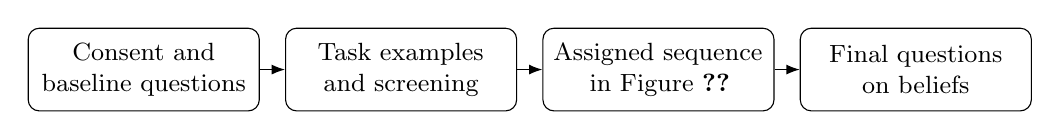
\begin{tikzpicture}[n/.style={draw,rounded corners,align=center,text width=2.7cm,minimum height=1.05cm,font=\small},>=Latex]
\node[n] (a) {Consent and\\baseline questions};
\node[n,right=.32cm of a] (b) {Task examples\\and screening};
\node[n,right=.32cm of b] (c) {Assigned sequence\\in Figure~\ref{fig:treeB}};
\node[n,right=.32cm of c] (d) {Final questions\\on beliefs};
\draw[->](a)--(b);\draw[->](b)--(c);\draw[->](c)--(d);
\end{tikzpicture}
\caption{\new{Common survey timeline. Professional characteristics precede the policy procedure; final belief reports follow the decisions. Policy ranking occurs at different points across arms.}}\label{fig:timelineB}
\end{figure}

\begin{figure}[!htbp]\centering\color{added}
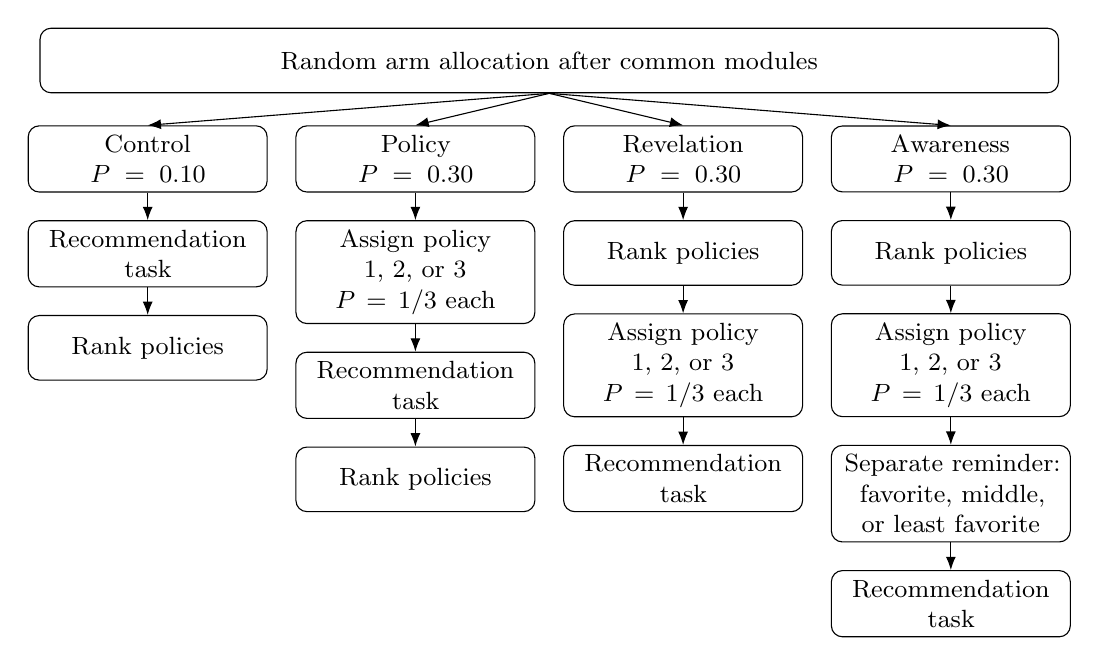
\begin{tikzpicture}[n/.style={draw,rounded corners,align=center,text width=2.8cm,font=\small,minimum height=.82cm},>=Latex]
\node[n,text width=12.7cm] (root) at (0,0) {Random arm allocation after common modules};
\node[n] (c) at (-5.1,-1.25) {Control\\$P=0.10$};
\node[n] (p) at (-1.7,-1.25) {Policy\\$P=0.30$};
\node[n] (r) at (1.7,-1.25) {Revelation\\$P=0.30$};
\node[n] (a) at (5.1,-1.25) {Awareness\\$P=0.30$};
\foreach \v in {c,p,r,a}{\draw[->](root.south)--(\v.north);}
\node[n,below=.35cm of c] (c1) {Recommendation\\task};
\node[n,below=.35cm of c1] (c2) {Rank policies};
\node[n,below=.35cm of p] (p1) {Assign policy\\1, 2, or 3\\$P=1/3$ each};
\node[n,below=.35cm of p1] (p2) {Recommendation\\task};
\node[n,below=.35cm of p2] (p3) {Rank policies};
\node[n,below=.35cm of r] (r1) {Rank policies};
\node[n,below=.35cm of r1] (r2) {Assign policy\\1, 2, or 3\\$P=1/3$ each};
\node[n,below=.35cm of r2] (r3) {Recommendation\\task};
\node[n,below=.35cm of a] (a1) {Rank policies};
\node[n,below=.35cm of a1] (a2) {Assign policy\\1, 2, or 3\\$P=1/3$ each};
\node[n,below=.35cm of a2] (a3) {Separate reminder:\\favorite, middle,\\or least favorite};
\node[n,below=.35cm of a3] (a4) {Recommendation\\task};
\foreach \u/\v in {c/c1,c1/c2,p/p1,p1/p2,p2/p3,r/r1,r1/r2,r2/r3,a/a1,a1/a2,a2/a3,a3/a4}{\draw[->](\u)--(\v);}
\end{tikzpicture}
\caption{\new{Vertical allocation and task sequence. Each treated policy cell has intended unconditional probability $0.30\times1/3=0.10$. The reminder is shown separately. Realized assigned and analyzed counts appear in Table~\ref{tab:flowB} and Appendix~\ref{app:cellsB}.}}\label{fig:treeB}
\end{figure}

\subsection{Policy content and recommendations}
The three scenarios are short descriptions of an educational environment under which teachers are asked to make their recommendations. Their English descriptions from the existing manuscript are retained in Appendix~\ref{app:policiesB}. Policy 1 promises small-group educational reinforcement with support staff. Policy 2 changes the evaluation-board procedure to unanimity for retention with secret and anonymous voting. Policy 3 provides tailored training and support in inclusive teaching and multilevel classroom management. No resources, evaluation-board voting rules, or staff training are actually implemented by assigning these descriptions.

The intended task presents eight student cards varying gender, complex background, failed subjects, basic competences, absence, and disciplinary problems. Each response recommends promotion or repetition. The existing inclusion rule excludes teachers recommending repetition for the favorable screening example. It does not exclude teachers declining repetition for the unfavorable example. We retain the established card coding and response sample: the two favorable-example fields are removed and other nonmissing recorded card responses are used. Most respondents therefore contribute eight or nine retained observations; some contribute fewer.

\new{This distinction matters more for treatment interpretation than for simple description. Introductory example responses precede assignment according to the study plan, and identifiers may be reused. The retained outcome is consequently a composite of collected recommendations, not a perfectly isolated mean of eight postassignment choices. An invariant preassignment component can dilute the measured treatment response; variable observation and profile composition can add further complications. We preserve the specified analysis rule but do not claim that profile adjustment recovers an unobserved postassignment-only outcome.}

\subsection{Analysis populations and outcome availability}
The raw export contains 4,942 records, including incomplete entries. Of these, 3,274 have an arm assignment: 337 Control, 984 Policy, 958 Revelation, and 995 Awareness. After the retained exclusion rules, 2,885 assigned records remain in the cleaned file, and 2,705 contribute a recommendation score. The remaining 180 retained assigned records have no usable recommendation. Table~\ref{tab:flowB} separates assignment, analytical retention, outcome availability, task-completion flags, and completion of the full survey.
\inputtab{added}{B_flow}{Assignment and availability of analysis outcomes}{tab:flowB}
\new{These indicators are not a single ordered survival sequence. Policy ranking is earlier in some arms, and a task-completion flag is not identical to retaining a usable outcome after exclusions. The assignment denominator is used for availability comparisons; rankings and final beliefs are not required for the main recommendation analysis. Ranking analyses use all retained respondents with the relevant ranking. In this export that rule produces the same 2,546 respondents as the intersection with score availability, but this equality is a property of the data rather than an imposed requirement.}

\section{Estimands and inference}
\subsection{Primary contrasts}
The main outcome is relative recommendation propensity. For teacher $j$, each recorded decision $Y_{ij}$ is compared with the leave-one-out repetition rate for the same card identifier, and these differences are averaged:
\[
 H_j=\frac{1}{n_j}\sum_{i\in I_j}(Y_{ij}-\bar Y_{i,-j}).
\]
The pooled reference standardizes for the cards observed. Multiplication by 100 expresses the result in percentage points. The main score sample does not condition on a policy ranking. A direct card-level analysis with card fixed effects and teacher-clustered errors provides a complementary specification.

The primary contrasts are Policy minus Control, Revelation minus Policy, and Awareness minus Revelation. The first compares an equally randomized mixture of the three assigned scenarios with no assigned scenario. The second changes ranking timing as well as prior exposure to all three policy descriptions. It is therefore the effect of that procedure, not an isolated effect of speaking a preference while holding information exposure constant. The third adds an explicit reminder after the same ranking-and-assignment sequence.

Unadjusted differences in teacher means are the primary estimates. Baseline-adjusted models use only the demographic and professional variables collected before the procedure. HC3 covariance accommodates heteroskedasticity at the teacher level. Teacher fixed effects cannot identify the main effect of an assignment that is constant within that teacher, so they are not added to these between-teacher regressions. There is no reliable school identifier for school-level clustering.

\new{Random assignment motivates intention-to-treat contrasts for an outcome observed for all assigned respondents. Here some outcomes are unavailable or excluded. The reported complete-observation differences follow assigned groups but are not automatically unbiased full-assignment ITT estimates. Their causal interpretation requires assumptions about selection and the recorded composite outcome. The availability comparisons, weighting sensitivity, and bounds below make this distinction explicit. A bootstrap with 1,999 assignment-universe teacher resamples reconstructs the profile reference, rather than treating the generated score as fixed throughout resampling.}

\subsection{Policy identities, preferences, and multiplicity}
We estimate the ten cell means and express all contrasts in a consistent direction. Within each treated arm, policies 2 and 3 are compared with policy 1. Within each policy, Revelation is compared with Policy and Awareness with Revelation. Two-by-three models provide joint tests of arm-by-policy interactions; additional joint tests compare the three policy identities within each arm. Individual contrast families use Holm adjustment \cite{holm}: three broad comparisons, nine treated cells versus control, six within-arm policy comparisons, and six between-arm comparisons within policy.

For Revelation and Awareness, preferences are elicited before policy assignment. We compare assignments to favorite and least-favorite policies against the middle-ranked policy, adjusting for favorite-policy identity, and test whether the reminder changes these contrasts. These estimates concern assignment to policy packages defined by prior rankings. Prior ranking does not randomize the underlying preference or separate policy content from alignment.

For Policy and Control, rankings follow the task. We retain the original ranking-adjusted and alignment-stratified specifications as secondary descriptions. Conditioning on a variable that may respond to assignment can change experimental comparisons \cite{post}. A small treatment coefficient on recommendations does not remove that concern. Later rankings are also analyzed as outcomes: for each policy, we compare the probability of ranking it first or last between respondents assigned to it and respondents assigned to another policy within the Policy arm, adjusting multiplicity over the six comparisons.

\subsection{Changes in academic criteria}
\begin{addition}
The mean comparison uses assignment between teachers. A separate comparison uses the multiple cards answered by each teacher to ask whether that assignment changes academic slopes. For each adjacent-arm pair, we estimate
\[
Y_{ij}=\alpha_j+X_{ij}'\beta+\gamma_F T_j F_{ij}+\gamma_C T_j C_{ij}+u_{ij},
\]
where $F$ denotes many failed subjects, $C$ low basic competences, and $T$ the first arm in the contrast. The six attributes enter $X$. A teacher fixed effect absorbs every characteristic constant within teacher, including the arm's main effect. It does not absorb $T_jF_{ij}$ or $T_jC_{ij}$ because the academic attributes change across that teacher's cards. Thus $\gamma_F$ compares the failed-subject slope between procedures; it is not the procedure's effect on the mean recommendation.

We cluster errors by teacher and adjust the six slope tests using Holm. Three additional joint tests, one per arm pair, test the two academic changes together and form their own Holm family. The interactions are a limited exploratory extension selected for their substantive role in the decision task. We also replace the six common attribute coefficients with exact-card fixed effects, and give every teacher equal total weight in a further specification. These checks assess whether the result depends on the additive profile adjustment or the number of responses. None identifies a psychological mechanism independently of the maintained coding, recorded-outcome definition and outcome-availability assumptions.
\end{addition}

\subsection{Precision and selection sensitivity}
We distinguish two summaries of the precision of a contrast.
\old{The first is the minimum detectable effect with 80 percent power. This tells us which effect sizes the design was able to detect with reasonable probability. The second is an equivalence test. This asks whether we can reject effects outside a given substantive margin.}
In the present reanalysis, MDEs are approximate sensitivity summaries calculated from the realized standard errors, not a substitute for prospective power calculations. Equivalence uses two one-sided tests at five percent, equivalent to checking whether a 90 percent interval lies inside a specified margin \cite{equivalence}. We report margins of two, three, and five percentage points. A three-point change corresponds to three additional recommendations per 100 comparable decisions, or about six percent of the observed teacher-average recommendation rate. Whether that is negligible depends on the purpose and costs of the policy. The two- and five-point margins show how conclusions change with a stricter or looser standard; none is asserted as a prospectively chosen smallest effect of interest. Individual equivalence tests are not simultaneous guarantees across every policy and subgroup.

\new{Availability models compare the probability of retaining a score, task completion, and survey completion across assigned arms and policies. Alignment-related availability is examined only where rankings precede policy assignment. Baseline balance comparisons use age, gender, experience, stage, and ownership, which are potentially observed among both retained and missing-outcome respondents. Final belief reports cannot diagnose selection among respondents who never reach them.}

\new{Two further analyses assess sensitivity to selection. Inverse-observation weighting uses baseline variables and assigned arm, with median replacement and missingness indicators for baseline omissions. It assumes selection is ignorable conditional on that information and sufficient overlap. The expanded bootstrap resamples teachers from the assignment universe 1,999 times, reconstructs the profile reference and reestimates the observation model and its weights in every draw. Baseline median imputations remain fixed. Percentile intervals therefore incorporate coefficient and weight estimation, conditional on that preprocessing and the selection model. Separately, worst-case bounds assign all missing outcomes either zero or one for the raw teacher-average binary recommendation measure. These require no missing-at-random assumption but concern a different outcome from $H_j$. We do not impose the monotonicity assumption required by Lee bounds across these procedures \cite{lee}.}

\new{We supplement extreme bounds with a gradual missing-outcome sensitivity for the raw teacher mean $H^a$. For each arm, an unobserved mean can differ from its observed mean by a specified amount. We vary these departures independently across the two arms, truncating means to $[0,1]$. This makes the selection assumptions needed to change the full-assignment mean contrast visible, without confusing them with confidence intervals for $H^b$.}

\section{Results}
\subsection{Average contrasts are small, with unequal precision}
Table~\ref{tab:broadB} reports the three primary comparisons. Policy minus Control is 0.62 points, with a 95 percent interval from $-2.27$ to 3.51. Revelation minus Policy is $-1.32$ points, with an interval from $-3.32$ to 0.67. Awareness minus Revelation is $-1.11$ points, with an interval from $-3.22$ to 1.00. None rejects a zero difference, with or without the broad-family multiplicity adjustment.
\inputtab{revised}{B_broad}{Primary recommendation contrasts and precision}{tab:broadB}
The three-point equivalence test yields a more discriminating conclusion. Policy versus Control does not pass: its 90 percent interval is [$-1.80$, 3.05] points. Revelation versus Policy passes narrowly, with [$-2.99$, 0.35], and Awareness versus Revelation passes with [$-2.88$, 0.66]. None of these three contrasts meets the tighter two-point margin; all meet the five-point margin under the primary HC3 specification. These are conditional observed-outcome conclusions, not evidence that all policy effects are exactly zero.
\plot{revised}{policy_broad}{Primary differences in relative recommendation propensity. Intervals are 95 percent; shading marks a three-point sensitivity margin. Equivalence decisions use 90 percent intervals.}{fig:broadB}
Baseline adjustment produces the same qualitative pattern of small estimates. In 1,999 bootstrap draws from the assignment universe, rebuilding the score reference gives 95 percent intervals of [$-2.03$, 3.45], [$-3.39$, 0.55], and [$-3.24$, 1.02] points. The 90 percent interval for Revelation minus Policy becomes [$-3.10$, 0.27], crossing the three-point margin. Only Awareness minus Revelation remains inside that margin in both the primary and expanded bootstrap analyses. The broad message is small mean estimates with sensitivity in narrow equivalence, rather than a robust qualitative separation between the two preference procedures.

\subsection{Policy-specific contrasts do not support a broad mechanism claim}
Figure~\ref{fig:cellsB} displays the ten mean outcomes; Table~\ref{tab:policiesB} groups the policy and arm contrasts. Policy 2 minus policy 1 within the Policy arm is approximately 2.13 points before conditioning on a later favorite ranking. The full pattern does not provide strong evidence of differences between policy identities: joint-test $p$-values are 0.423, 0.885, and 0.928 in Policy, Revelation, and Awareness. Joint arm-by-policy interaction tests give $p=0.785$ for Revelation versus Policy and $p=0.949$ for Awareness versus Revelation.
\plot{revised}{policy_cells}{Mean relative recommendation propensity in the ten assignment cells, with HC3 95 percent intervals. These are levels relative to pooled profile benchmarks, not differences from control.}{fig:cellsB}
\inputtab{revised}{B_policy_contrasts}{Policy identity and procedure comparisons}{tab:policiesB}
The ranking-adjusted specification for policy 2 yields Revelation minus Policy of $-3.04$ points (95 percent interval $-6.24$ to 0.15; unadjusted $p=0.062$). Its direction is toward lower, not higher, relative recommendation propensity under Revelation. Because the specification includes a ranking observed at different times, and the contrast is one among several, it cannot establish a mechanism of resistance or acceptance. The complete unadjusted cell comparisons are the clearer starting point for interpretation.

\subsection{Small average changes coexist with a change in the failed-subject slope}
\begin{addition}
Table~\ref{tab:slopesB} reports the six academic-slope contrasts. Scenario assignment versus control produces changes close to zero for both indicators. Earlier preference elicitation increases the failed-subject slope by 3.72 points and reduces the low-competence slope by 1.96 points, with neither individual contrast clear after multiplicity adjustment. Adding the reminder then changes the two slopes by $-4.98$ and 2.72 points, respectively.
\end{addition}
\inputtab{added}{B_academic_slopes}{Procedure differences in the use of academic information}{tab:slopesB}
\begin{addition}
The reminder's failed-subject contrast has a 95 percent interval of [$-8.47$,$-1.50$] and a six-test Holm $p$ of 0.031. Its direction means that the gap in recommendations between profiles with many and few failed subjects is smaller under Awareness than under Revelation. It does not mean that Awareness reduces recommendations by five points for every profile, or that academic failures cease to dominate decisions.

The joint test of both academic changes yields $p=0.019$ before and 0.058 after correction across the three arm-pair tests. The distinction is relevant: one component has clearer evidence than the broader claim that the vector of academic weights changes. Exact-card fixed effects give a failed-subject contrast of $-4.97$ points; adding inverse response-count weights gives $-4.88$ points. The point estimate is therefore not sensitive to those two modeling choices, although these are robustness checks on the same data rather than independent confirmations.

This is an exploratory qualification to the mean results. Making preference alignment explicit may alter how respondents apply an academic criterion even when the average composite barely moves. The data do not establish whether this reflects greater consideration of alternatives, consistency with stated views, task framing, or another response process. They also do not demonstrate that the reminder improves decision quality. The mean contrasts alone therefore do not settle whether academic criteria change.
\end{addition}

\subsection{Prior alignment and later preference reports answer different questions}
Among teachers who rank policies before assignment, favorite versus middle-ranked assignment is associated with 2.23 points in Revelation and 1.13 points in Awareness. Their 95 percent intervals are [$-1.05$, 5.51] and [$-2.31$, 4.57]. Least-favorite versus middle-ranked assignment gives 0.21 and 1.58 points, respectively, also with intervals spanning zero. The joint interaction test for changing these alignment contrasts with the reminder gives $p=0.583$. These comparisons do not tightly exclude all substantively relevant alignment responses.
\inputtab{added}{B_alignment}{Alignment using preferences elicited before policy assignment}{tab:alignB}
In contrast, reported preferences are not uniformly insensitive to assignment. Within Policy, 761 retained respondents provide a ranking. Assignment to teacher training raises its subsequent first-place ranking probability by 9.76 points, with a 95 percent interval from 2.50 to 17.01. The Holm-adjusted $p$-value is 0.0507 across six first/last-place outcomes. Its last-place ranking falls by 5.85 points, with an interval narrowly including zero. Table~\ref{tab:prefB} presents the complete family so that this finding is not selected in isolation.
\inputtab{revised}{B_preferences}{Assigned policy and its subsequent ranking in the Policy arm}{tab:prefB}
\new{The estimated ranking response is substantively larger than the mean recommendation contrasts, although the outcomes and scales capture different behavior. Its adjusted $p$ of 0.0507 indicates uncertainty near a conventional threshold; it should not be converted into a sharp distinction between an established effect and no response. The result is compatible with changed valuation or response consistency, without separating them. It is not necessary to establish a definitive ranking effect to recognize that a later ranking is potentially posttreatment. Conversely, the null average recommendation contrasts do not constitute a test of invariance in preferences.}

\begin{addition}
The complete ranking distributions help interpret what changes and what remains common across procedures (Table~\ref{tab:ranksharesB}). Reinforcement is the most frequently favored scenario: 51.6--58.4 percent place it first across arms. Unanimity and secret voting are most frequently ranked last: 72.0--78.4 percent. Training is generally intermediate, with first-place shares of 30.8--39.3 percent. This pattern suggests stronger stated support for capacity-building descriptions than for the collective promotion-rule description, but it is not a preference between experimentally isolated policy features.

None of the 18 adjacent-arm first/last-place contrasts is clear after a common Holm adjustment. The raw distributions are also measured at different points in the procedure: rankings in Revelation and Awareness precede policy assignment and the reminder. Their difference cannot be attributed to receiving the reminder. The within-Policy assignment contrast instead concerns a genuinely later ranking. Keeping these comparisons separate avoids treating timing differences as a common posttreatment preference outcome.
\end{addition}
\inputtab{added}{B_ranking_shares}{Favorite and least-favorite policies across procedures}{tab:ranksharesB}

\subsection{Outcome availability and robustness delimit the interpretation}
The probability of observing a retained score is 83.38 percent in Control, 83.74 percent in Policy, 82.46 percent in Revelation, and 81.41 percent in Awareness. The corresponding adjacent-arm differences are 0.36, $-1.28$, and $-1.06$ points, with 95 percent intervals spanning zero. These similarities do not prove ignorable selection. Teachers with an observed retained score are younger than assigned respondents without one (45.06 versus 48.82 years) and have less experience (16.85 versus 20.24 years). These differences combine the retained screening rule and missing responses; they should not all be attributed to quitting the survey.

\new{Inverse-observation-weighted estimates are 0.64, $-1.27$, and $-1.15$ points, close to the primary results under the weighting assumptions. Symmetrically trimming the fastest and slowest 1.75 percent by total recorded duration also leaves small broad-arm estimates. Total duration may include time away from the survey, so trimming is a sensitivity analysis rather than a preferred attention rule. A card-level model with exact-profile effects and inverse response-count weights gives 0.64, $-1.25$, and $-1.07$ points. Its close agreement with the teacher-level contrasts shows that equal teacher weighting reconciles much of the difference from the unweighted card-level model. Appendix tables report both the weighting comparison and bootstrap intervals with reestimated selection weights.}

The assumption-free bounds are much wider. For the raw mean recommendation outcome, Policy minus Control lies between $-15.54$ and 17.34 points under extreme assignments of missing outcomes; the other adjacent-arm bounds are [$-17.33$, 16.46] and [$-18.72$, 17.41]. These are identification bounds, not confidence intervals. Their width makes clear that similar observed availability rates do not establish small full-assignment effects without restrictions on the unobserved recommendations.

\section{Discussion}
The experiment distinguishes three dimensions of responsiveness to policy messages: average recommendations, the application of academic criteria, and stated support. Average composite contrasts are small and do not reject zero, while narrower statements of equivalence depend on the procedure and inferential method. The criterion analysis identifies an exploratory reduction in the failed-subject slope with the alignment reminder. The later-ranking analysis suggests that assignment can also influence reported policy support. These findings require a more differentiated interpretation than either policy effectiveness or teacher resistance.

\new{A change in criteria is conceptually distinct from a change in the mean. Teachers can attach a different marginal importance to failed subjects while other signals, offsets across profiles, or the recorded response composition leave the aggregate little changed. The slope result is stable to exact-card effects and equal teacher weights, but its exploratory status and the weaker adjusted joint test limit how strongly to generalize it. The evidence supports reporting the signal and its boundaries, not building an unverified mechanism around it.}

The policy content further limits what recommendations can establish. Reinforcement does not supply an actual support teacher, and the training message does not increase instructional skill. The unanimity scenario changes a collective decision rule whose implementation could alter retention without changing an individual's preferred recommendation at all. Small individual mean responses therefore do not establish that these institutional channels are ineffective. Equally, the strong preference for reinforcement and rejection of the voting-rule scenario do not measure their causal educational benefits.

Preference timing has both substantive and methodological implications. Earlier elicitation exposes respondents to the menu and asks them to commit to an ordering; the additional reminder makes an already elicited alignment explicit. Later rankings can change with exposure or response consistency and should be analyzed as outcomes rather than automatically controlled as baseline preferences. Earlier rankings support conditional assignment comparisons, but favorite-policy assignment remains a bundle of policy identities and personal rankings, not an isolated psychological treatment of liking.

\new{Precision also has several layers. For observed composite means, the data exclude some large average differences under the specified estimators. They do not uniformly establish effects smaller than three points, particularly for prior elicitation when references are rebuilt in the expanded bootstrap. Specific policy and alignment comparisons are less precise. For the full assignment universe, missing outcomes permit much wider differences without assumptions, and the gradual sensitivity display shows which departures from observed means would change the sign or size of those contrasts. Reestimated inverse-observation weights address observed selection under a model; they do not resolve selection on unmeasured recommendations.}

The main measurement limitation is that the retained response definition includes example information and cannot perfectly separate reused question instances. This can dilute responsiveness and complicate the interpretation of the composite as a postassignment outcome. Recruitment is voluntary and regional, and reliable school-level clustering is unavailable. These limitations are most important for extending the results to implementation or populations beyond the observed respondents. Within those boundaries, the experiment provides evidence on several dimensions of response that should not be collapsed into a single null-policy conclusion.

\section{Conclusion}
Brief scenarios and preference procedures yield small mean contrasts in recorded repetition recommendations, but that is not the whole response pattern. An exploratory reminder contrast indicates less weight on failed subjects, and exposure to the training scenario is associated with greater subsequent stated support. The evidence is uneven across these dimensions and remains sensitive to measurement and selection. The paper's contribution is to distinguish them explicitly: policy endorsement, decision criteria and average recommendations are related outcomes, not interchangeable measures of teacher responsiveness.

\clearpage\begingroup\color{revised}\begin{thebibliography}{99}\small
\bibitem{allen} C. S. Allen, Q. Chen, V. L. Willson, and J. N. Hughes, ``Quality of research design moderates effects of grade retention on achievement: A meta-analytic, multilevel analysis,'' \textit{Educational Evaluation and Policy Analysis}, vol. 31, no. 4, pp. 480--499, 2009. \href{https://doi.org/10.3102/0162373709352239}{doi:10.3102/0162373709352239}.
\bibitem{goos} M. Goos, J. Pipa, and F. Peixoto, ``Effectiveness of grade retention: A systematic review and meta-analysis,'' \textit{Educational Research Review}, vol. 34, art. 100401, 2021. \href{https://doi.org/10.1016/j.edurev.2021.100401}{doi:10.1016/j.edurev.2021.100401}.
\bibitem{tomchin} E. M. Tomchin and J. C. Impara, ``Unraveling teachers' beliefs about grade retention,'' \textit{American Educational Research Journal}, vol. 29, no. 1, pp. 199--223, 1992. \href{https://doi.org/10.3102/00028312029001199}{doi:10.3102/00028312029001199}.
\bibitem{bonvin} P. Bonvin, ``The role of teacher attitudes and judgement in decision-making: The case of grade retention,'' \textit{European Educational Research Journal}, vol. 2, no. 2, pp. 277--294, 2003. \href{https://doi.org/10.2304/eerj.2003.2.2.6}{doi:10.2304/eerj.2003.2.2.6}.
\bibitem{klapproth} F. Klapproth and C. Beyte, ``GPA, student gender, school subject, and teacher attitudes in grade retention decisions: An experimental study,'' \textit{European Journal of Psychology of Education}, vol. 41, art. 24, 2026. \href{https://doi.org/10.1007/s10212-026-01072-7}{doi:10.1007/s10212-026-01072-7}.
\bibitem{kunda} Z. Kunda, ``The case for motivated reasoning,'' \textit{Psychological Bulletin}, vol. 108, no. 3, pp. 480--498, 1990. \href{https://doi.org/10.1037/0033-2909.108.3.480}{doi:10.1037/0033-2909.108.3.480}.
\bibitem{pajares} M. F. Pajares, ``Teachers' beliefs and educational research: Cleaning up a messy construct,'' \textit{Review of Educational Research}, vol. 62, no. 3, pp. 307--332, 1992. \href{https://doi.org/10.3102/00346543062003307}{doi:10.3102/00346543062003307}.
\bibitem{spillane} J. P. Spillane, B. J. Reiser, and T. Reimer, ``Policy implementation and cognition: Reframing and refocusing implementation research,'' \textit{Review of Educational Research}, vol. 72, no. 3, pp. 387--431, 2002. \href{https://doi.org/10.3102/00346543072003387}{doi:10.3102/00346543072003387}.
\bibitem{holm} S. Holm, ``A simple sequentially rejective multiple test procedure,'' \textit{Scandinavian Journal of Statistics}, vol. 6, no. 2, pp. 65--70, 1979. \url{https://www.jstor.org/stable/4615733}.
\bibitem{post} J. M. Montgomery, B. Nyhan, and M. Torres, ``How conditioning on posttreatment variables can ruin your experiment and what to do about it,'' \textit{American Journal of Political Science}, vol. 62, no. 3, pp. 760--775, 2018. \href{https://doi.org/10.1111/ajps.12357}{doi:10.1111/ajps.12357}.
\bibitem{equivalence} D. Lakens, ``Equivalence tests: A practical primer for t tests, correlations, and meta-analyses,'' \textit{Social Psychological and Personality Science}, vol. 8, no. 4, pp. 355--362, 2017. \href{https://doi.org/10.1177/1948550617697177}{doi:10.1177/1948550617697177}.
\bibitem{lee} D. S. Lee, ``Training, wages, and sample selection: Estimating sharp bounds on treatment effects,'' \textit{Review of Economic Studies}, vol. 76, no. 3, pp. 1071--1102, 2009. \href{https://doi.org/10.1111/j.1467-937X.2009.00536.x}{doi:10.1111/j.1467-937X.2009.00536.x}.
\end{thebibliography}
\endgroup
\clearpage\appendix\let\originalsection\section\renewcommand{\section}{\sectionfloatbarrier\originalsection}
\section{Policy descriptions}\label{app:policiesB}
The following English descriptions preserve the wording in the existing manuscript. Numeric labels in the analysis correspond to A, B, and C respectively.
\begin{enumerate}
\item \old{\textbf{Policy A: Educational reinforcement.} The student will receive educational reinforcement in a small group next school year, with a support teacher, inside or outside the classroom.}
\item \old{\textbf{Policy B: Modified promotion criteria.} The promotion criteria will be modified in the Evaluation Board: unanimity for grade retention, secret and anonymous voting.}
\item \old{\textbf{Policy C: Teacher training.} All school staff will receive tailored training and teaching support in inclusive teaching methodologies and multi-level classroom management.}
\end{enumerate}
\new{The questionnaire asks respondents to rank the three policies from favorite to least favorite. The initial display order is randomized according to the study plan. In Awareness, the reminder reports whether the assigned policy occupies the favorite, middle, or least-favorite position. The relevant intervention is the presence of this reminder, conditional on the earlier assigned arm; its content is not a separately randomized treatment.}

\section{Cell counts, availability, and selection}\label{app:cellsB}
\inputtab{added}{B_cells_flow}{Realized policy-cell sample sizes}{tab:cellflowB}
\begin{addition}
The assignment universe is defined by a nonmissing valid treatment code in the raw export, not by completion of the final page. Screening retention, availability of a score, ranking availability, and the survey-finished flag are retained as separate indicators. Table~\ref{tab:availabilityB} shows availability contrasts from this universe. Comparisons of attrition by alignment are restricted to Revelation and Awareness respondents with an earlier ranking; they do not condition on later rankings from Policy. Conditional denominators for those contrasts are documented in the aggregate replication tables.
\end{addition}
\inputtab{added}{B_availability}{Differences in retained-score availability from assignment}{tab:availabilityB}
\inputtab{added}{B_balance}{Baseline characteristics by retained-score availability}{tab:balanceB}
\plot{added}{availability_by_arm}{Availability of recorded indicators relative to initial assignment. Connecting lines facilitate comparison of indicators; they are not survival curves, because ranking occurs at different points across arms.}{fig:availabilityB}
\new{The replication package contains all policy-by-arm and prior-alignment availability regressions, with their own denominators. Availability outcomes are not collapsed into a Cox model because task order differs across arms and total elapsed time is not a consistent measure of time at risk. Identification bounds use the observed fraction $r_a$ and observed mean $\bar Y_a$ in arm $a$: the arm mean is bounded by $[r_a\bar Y_a,r_a\bar Y_a+1-r_a]$. A difference takes the lower endpoint of one arm minus the upper endpoint of the other, and conversely.}

\section{Alternative specifications and precision}
\inputtab{revised}{B_sensitivity}{Primary contrasts under alternative specifications}{tab:sensB}
The card-level specification includes card fixed effects and clusters errors by teacher. It gives more weight to teachers with more recorded responses, unlike the teacher-level mean comparison. The baseline-adjusted specification conditions on professional characteristics observed before the policy procedure. Neither includes teacher fixed effects for the main assignment contrast. Bootstrap draws resample teachers and reconstruct leave-one-out profile rates. These procedures examine different sources of sensitivity and should not be interpreted as independent replications.
\inputtab{added}{B_weighted_profiles}{Exact-profile adjustment with equal teacher weights}{tab:weightedB}
\inputtab{added}{B_refitted_bootstrap}{Reconstructed-reference and reestimated-weight bootstrap intervals}{tab:bootB}
\begin{addition}
The bootstrap resamples all 3,274 assigned records with replacement, allowing both observed counts and composition to vary. An observed teacher selected multiple times contributes that multiplicity to every card total. Each bootstrap copy's leave-one-out rate excludes its own response, rather than excluding all copies of the original teacher. The selection logit is reestimated using assignment multiplicities, arm, baseline characteristics and their missingness indicators; inverse probabilities are bounded using a 0.05 floor. No inferential claim of ignorability follows from the similarity of point estimates.

For the gradual missing-outcome display, let $r_a$ be the observed fraction and $\mu_a$ the observed $H^a$ mean in arm $a$. A hypothesized full-assignment mean is
\[
M_a(\delta_a)=r_a\mu_a+(1-r_a)\max\{0,\min[1,\mu_a+\delta_a]\}.
\]
We vary each arm's $\delta$ independently between $-0.30$ and 0.30 and plot $M_a(\delta_a)-M_b(\delta_b)$. The origin assumes missing respondents have their own arm's observed mean. Moving along one axis relaxes that assumption in one arm; a common movement along both axes need not cancel because availability fractions differ. The contour is the zero contrast, not a confidence boundary. The exercise concerns $H^a$, avoiding an assumption that the profile-adjusted $H^b$ is bounded by zero and one.
\end{addition}
\plot{added}{missing_outcome_grid}{Full-assignment raw-mean contrasts under independent departures of missing from observed outcomes. Axis units are percentage points; colors show the hypothesized contrast and the black line marks zero. These are selection scenarios, not estimates of the missing responses.}{fig:missingB}

\inputtab{added}{B_equivalence}{Equivalence sensitivity for the broad-arm contrasts}{tab:eqB}
\new{The minimum detectable effects in Table~\ref{tab:broadB} use $(t_{.975}+t_{.80})\widehat{SE}$, approximately, for two-sided five-percent testing. They describe realized precision. Equivalence margins are expressed on the recommendation-probability scale: a three-point margin is neither three percent of the baseline rate nor three percent of a standard deviation. The family-specific Holm corrections apply to difference tests; individual equivalence conclusions are reported separately and do not certify that every subgroup is equivalent.}

\section{Academic criteria and the full ranking comparisons}
\inputtab{added}{B_academic_robust}{Robustness of the procedure-by-academic contrasts}{tab:sloperobB}
\inputtab{added}{B_ranking_contrasts}{Complete adjacent-arm comparisons of favorite and least-favorite rankings}{tab:rankcontrastsB}
\new{The exact-card specifications absorb common differences between identifiers, including common attribute interactions not represented by an additive six-attribute model. Teacher effects remain in these slope specifications because the target is a difference in within-teacher criteria. This differs from the mean-assignment model, which cannot include teacher effects. No significance search over additional teacher subgroups is used to select the reported academic contrasts.}

\section{Secondary alignment and ranking-adjusted analyses}
\inputtab{revised}{B_secondary_alignment}{Secondary comparisons conditioning on reported alignment}{tab:secondaryB}
These specifications retain the original comparative structure, including comparisons to Control for favorite and least-favorite assignments in Policy and comparisons across successive arms within alignment categories. Where a ranking follows assignment or decisions, they are descriptive rather than the primary causal contrasts. The preferred temporal comparison for the reminder uses Revelation and Awareness with their preassignment ranking and the joint interaction test reported in the main text.

\inputtab{added}{B_alignment_precision}{Precision of all retained alignment comparisons}{tab:alignprecisionB}
\new{Equivalence is evaluated for the full retained set of alignment comparisons, including descriptive comparisons based on later rankings. It does not repair their timing or confer causal interpretation. MDEs summarize realized precision; they are not retrospective probabilities that the null is true. The displayed individual margins also do not constitute a joint equivalence statement over the collection of policies, ranks and procedures.}

\section{Scope, plan, and replication disclosure}
\begin{addition}
The companion manuscript \textit{Shared Academic Criteria and Systematic Disagreement in Teachers' Grade-Repetition Recommendations} uses the same survey to study within-teacher attribute patterns, same-profile disagreement, and held-out prediction. The present paper uses attribute interactions only to study differences induced by the assigned procedures, rather than claiming the companion paper's overall attribute and disagreement results as a separate contribution. Editors and readers should evaluate the overlap with that shared dataset disclosed.

The local initial analysis plan describes the treatment structure and hypothesis families. The current organization, main sample definitions by objective, multiplicity summaries, selection diagnostics, and precision sensitivity analyses are part of a subsequent reanalysis. A public time-stamped registration is not asserted on the basis of the local PDF alone. The analysis scripts and aggregate outputs accompany the working manuscripts in a separate directory; the original manuscript and its results are preserved. Research-governance and data-release declarations require verification from the study records before journal submission.
\end{addition}
\end{document}
